\chapter{相关技术背景}
我们所调研的开放式关系抽取,是从未指定的随机领域的中文文本语料库中对实体间不定类型关系的抽取,抽取结果为未指定的关系的实体间关系元组。这一个章节将介绍所调研出的对于中文开放式关系抽取主流技术。第一部分将讨论当前主流中文开放式关系抽取系统中对文本数据分析的预处理阶段所涉及到的自然语言处理过程,即标注词性,依存分析与分割词汇。之后的部分以兼词处理为中心,讨论对候选关系元组抽取的过程\citep{liyang2016}。

\section{中文分词}
\subsection{概述}
分词,即分割词汇,是将输入的语料库中的源文本按照所给的规则对句子进行切割,以将语句分割为逐个正确组合的、可以获取其含义的单词序列过程。当前流行的分析系统大部分都是英文语境下的分词,而英文单词之间以显示的空格进行分离,中文却没有如此显示分割,是以互相独立的中文单字组成,由其组成的词语是中文语境下可以获取语义的最小单位。特别是在现实生活中,中文词汇所含中文单字的数量没有规律,最小情况下一个单字就可以构成词语,也有上不封顶的成语词,故中文语境下的分词难度远大于英文语境下的分词。

\subsection{中文分词研究现状}
\subsubsection{字符串匹配分词法}
提供所需的分词字典和规则是这种方法的前提,其工作原理就是字符串匹配,把输入的源文本与所提供的字典里的词汇进行匹配,若匹配成功则将这个词汇从源文本中分割出来作为分词的输出,反之则不分割。这种方法简单粗暴,易于实现,但是如果源文本出现词典中未提供的新词语,并且新词汇的出现是必然的,分词输出的错误将无法避免。类似于字符串匹配,这种分词的办法也有正逆向和根据匹配长度的最大、最小匹配的算法。

\subsubsection{基于规则的分词法}
这种分词的办法基于语言学,让计算机对人理解语句和分析语句含义的过程进行模拟,进而达到对语句分词的效果,这种分词模块的构造包括知识库与推理机,二者分别涉及到极大的构造工作量、极大的难度与艰深的推理过程,故难以实现。

\subsubsection{统计分词法}
这种分词的方法基于假设:词汇是一种稳定的中文单字顺序结构,即有着十分巨大的语料库的前提下,一些特定中文单字顺序结构出现的频率如果超过一定的阈值,则可以假设这种中文单字的顺序结构是一个词汇。也就是说,将语料库当中相邻出现的中文单字组合逐个记录出现频率,依据统计结果可以得出每一个组合是一个词汇的概率。

这种方法需要基于一定规模的语料库,所以需要大量的数据。但是根据分词统计模型来得出各种中文单字顺序结构是一个词汇的概率,这种方法解决了前两种方法存在的问题:难以识别多义词与难以识别未知词(即未把词汇加入词典)。

\section{词性标注}
\subsection{概述}
词性即词的性质,代表词的语法功能。是其类别的归类,在指定的词汇类别系统里。对于中文文本中的词汇,词性由其所处语句的上下文与被指定的词汇类别系统所决定。而词性标注即根据上下文,确定词汇的合理的词性(动词,名词等)从而可以对词汇进行结果的标注。

中文语境下的词汇的词性随着上下文语境的变化而变化,即中文词汇存在着词性兼类现象,同一个中文词汇可能会有着数个不相同的词性。所以中文语句的词性标注另一个主要问题,语句中可能出现的词性兼类现象导致可能会出现错误标注。

\subsection{研究现状}

\begin{table}[htbp]
\centering
\caption[词性标注方法对比]{各种词性标注方法的对比} \label{tab:simpletable}
\begin{tabular}{|c|c|c|c|}
    \hline
    方法名 & 准确率 & 时间复杂度 & 实用性 \\
    \hline
    基于规则的方法 & 低 & 低 & 低 \\
    \hline
    基于统计的方法 & 较高 & 较高 & 中 \\
    \hline
    统计与规则的混合方法 & 较低 & 高 & 高 \\
    \hline
\end{tabular}
\end{table}

\subsubsection{基于规则的方法}
这种方法需要基于中文的语法特征来构造规则,再根据已经定义好的规则标注未处理的源文本的词性类别。该方法的缺点显而易见,在提前构造规则时需要消耗大量的人工,并且很难做到面面俱到,还需要规则建立者对语言学有透彻的理解以让规则准确而简洁,难以保证规则的普适性,并且随着规则的不断增加,有可能发生冲突。故需要预先权衡规则的广度与精度。

\subsubsection{基于统计的方法}
这种方法根据通过对一定规模的语料库进行分析、归纳所取得的统计数据,以未标注词汇序列所在的上下文环境计算其所属词性的概率。这种办法相对于上一个方法减少了人工工作量,且避免了人的主观性,体现了以数据说话的客观性,可是由于其模型的信息是由对语料库进行统计获得的,所以时间复杂度较高,并且准确性依赖于训练数据集的规模,规模越大则准确性越高。

\subsubsection{统计与规则的混合方法}
这种方法显而易见,是上面两种方法的结合,即首先通过较高数量的训练数据集训练之后计算得出统计模型,再以人工从训练数据集里总结规律,构造规则,再同时以统计模型与人工构造的规则标注源文本的词汇的词性。

\subsection{兼类词}
兼类词即多义词,例如“水”,既可以是名词(喝水),也可以是形容词(这次考试很水)。对于单性词,标注词性只需要词典即可,但兼类词在不同的上下文中有着不同的语义,所以兼类词的词性标注基于上下文的匹配性。兼类词在中文里的使用十分频繁,主要有形容词名词混用、动词形容词混用、名词动词混用。

\section{依存句法分析}
\subsection{概述}
依存句法分析可以得出待分析句子的句法结构,工作方式为分析词汇之间的依存方式,主要目的为识别语句中的各种语法成分(主谓宾,定状补等)并分析存在于各个句子元素当中的关系,其中动词作为核心词,独立于其他语句中的元素,不受到影响。

\begin{figure}[ht]
\centering
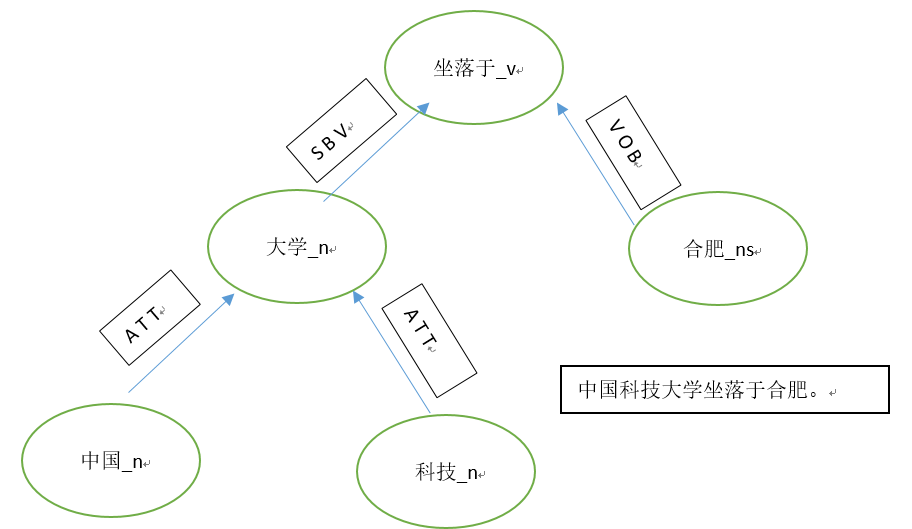
\includegraphics[width=13cm]{dependency}
\caption[依存分析样例]{依存分析样例}\label{fig:dependency}
\end{figure}

依存关系就是词汇中互相存在的关系。当中存在两个类型的词汇修饰词与核心词。以 $sen = w_0w_1...w_n$ 代表依存分析的输入句子,$w_i$ 即句子内第 $i$ 个词汇,$d = \{ \left( h,m,r\right) :0\leq h\leq n,1\leq m\leq n,r\in R \}$ 代表依存树,以 $w_h, w_m$ 分别表示核心词与修饰词,$\left( h,m,r\right)$ 表示 $w_h$ 到 $w_m$ 的依存关系,$r$ 则为二者的关系类型,$R$ 为 $r$ 的集合,即关系集合。

\subsection{研究现状}
通常情况下,当前的依存句法分析主流方法有基于转移方法和基于图模型方法,前者求解速度更快,但不能在长距离依存上良好的工作;而后者则在全部的结果集里搜索最优解,不受依存距离影响,可是有着高时间复杂度与低效率,。

\subsubsection{基于图模型方法}
这个方法工作原理是从输入语句转化的完全有向图内寻找拥有着最高的概率的依存树,从而构造出依存树并进行分析。图的搜索算法的性能需要下列前提满足才能较高:语句转化的依存树内的子树里的依存关系互相影响,独立于子树外的依存关系。这个方法目前面临的最大问题是如果模型中加入了更多特征,则系统复杂度将会提高,而当前的主流解决方法为在加入更多特征时削减满足图搜索算法性能的前提条件。

\subsubsection{基于转移方法}
这个方法将分析语句的方向设为从左到右,即一个动作序列。不同的动作序列将会生成不同的依存树结构。故搜索最优动作序列便可以构造出最优依存树。这个方法可以比上面的方法更加快捷地增添新特征。该方法的求解时间是线性的,故系统的效率降低与增添新特征仅存在微小的联系。

\section{本章小结}
这一章的内容集中于对中文语境下各种分词、词性标注、依存句法分析的各类方法的概述与其研究现状的调研,帮助理解作为关系抽取最重要的准备工作的自然语言处理过程中各项细节的技术。